
\section{Ejercicio 1}
\subsection{Introducción}

\subsection{Desarrollo}


\subsection{Correctitud}



\subsection{Complejidad}

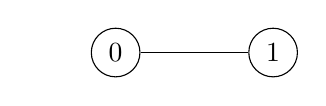
\begin{tikzpicture}
\node(pseudo) at (-1,0){};
\node(0) at (0,0)[shape=circle,draw]        {$0$};
\node(1) at (2,0)[shape=circle,draw]        {$1$};
\path [-]
  (0)      edge                 node [above]  {}     (1);

\end{tikzpicture}

%Pongo los tests que hice por si acaso.
\begin{table}[H]
\begin{center}
\begin{tabular}{|l|l|}
\hline
Materias & Aulas en las que se puede dictar \\
\hline \hline
0 & (1, 2) \\ \hline
1 & (1) \\ \hline
\end{tabular}
\end{center}
\end{table}

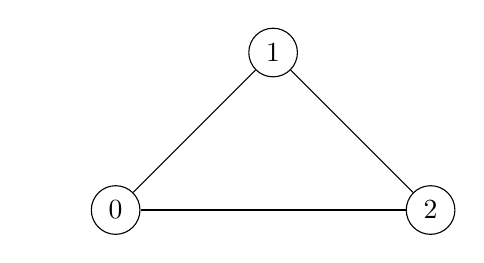
\begin{tikzpicture}
\node(pseudo) at (-1,0){};
\node(0) at (0,0)[shape=circle,draw]        {$0$};
\node(1) at (2,2)[shape=circle,draw]        {$1$};
\node(2) at (4,0)[shape=circle,draw]        {$2$};
\path [-]
  (0)      edge                 node [above]  {}     (1)
  (1)      edge                 node [above]  {}     (2)
  (2)      edge                 node [above]  {}     (0);
\end{tikzpicture}


\begin{table}[H]
\begin{center}
\begin{tabular}{|l|l|}
\hline
Materias & Aulas en las que se puede dictar \\
\hline \hline
0 & (1, 3) \\ \hline
1 & (2) \\ \hline
2 & (1, 2) \\ \hline
\end{tabular}
\end{center}
\end{table}

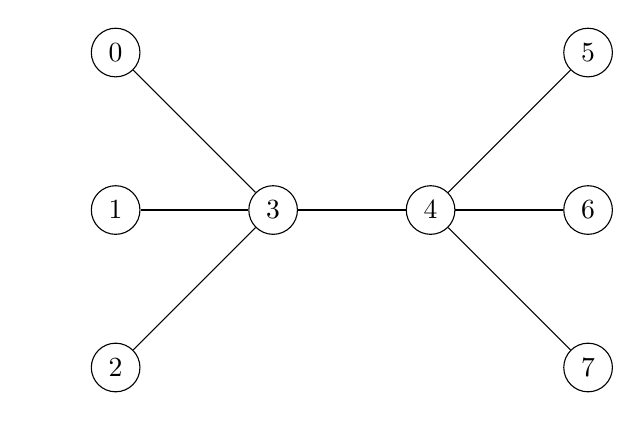
\begin{tikzpicture}
\node(pseudo) at (-1,0){};
\node(0) at (0,2)[shape=circle,draw]        {$0$};
\node(1) at (0,0)[shape=circle,draw]        {$1$};
\node(2) at (0,-2)[shape=circle,draw]        {$2$};
\node(3) at (2,0)[shape=circle,draw]        {$3$};
\node(4) at (4,0)[shape=circle,draw]        {$4$};
\node(5) at (6,2)[shape=circle,draw]        {$5$};
\node(6) at (6,0)[shape=circle,draw]        {$6$};
\node(7) at (6,-2)[shape=circle,draw]        {$7$};
\path [-]
  (0)      edge                 node [above]  {}     (3)
  (1)      edge                 node [above]  {}     (3)
  (2)      edge                 node [above]  {}     (3)
  (3)      edge                 node [above]  {}     (4)
  (4)      edge                 node [above]  {}     (5)
  (4)      edge                 node [above]  {}     (6)
  (4)      edge                 node [above]  {}     (7);
\end{tikzpicture}


\begin{table}[H]
\begin{center}
\begin{tabular}{|l|l|}
\hline
Materias & Aulas en las que se puede dictar \\
\hline \hline
0 & (1, 4) \\ \hline
1 & (2, 3) \\ \hline
2 & (3, 4) \\ \hline
3 & (4, 3) \\ \hline
4 & (1, 3) \\ \hline
5 & (2, 1) \\ \hline
6 & (3, 4) \\ \hline
7 & (4, 1) \\ \hline
\end{tabular}
\end{center}
\end{table}

\subsection{Experimentación}




